% !TEX root = ../main.tex
\section{Notations and Preliminaries}\label{sec:prelim}

% \subsection{Path decomposition}
\subsection{Basic definitions}
\begin{definition}[Path Decomposition \cite{cygan2015parameterized}]\label{def:path_dec}
A \textit{path decomposition} of a graph $G = (V, E)$ is a sequence of bags $\mathcal{P} = \{X_1, \dots, X_r\}$, where each $X_i \subseteq V$ such that following conditions hold:
\begin{enumerate}
	\item For each $v \in V$, there exists a pair of indices 
	$1 \leq l(v) \leq r(v) \leq r$ such that 
	\[v \in X_i \Longleftrightarrow l(v) \leq i \leq r(v).\]
	In other words each graph vertex maps to continuous subpath of the decomposition.   
	\item For each $uv \in E$, there exists an $i$ such that $\{u, v \} \subseteq X_i$.
\end{enumerate}

\end{definition}
\begin{definition}[Nice Path Decomposition \cite{cygan2015parameterized}]\label{def:nice_path_dec}
A \textit{nice path decomposition} is a path decomposition, where additional conditions hold:
\begin{enumerate}
	\item $X_1, X_r = \varnothing$.
	\item Each bag, except $X_1$, either \textit{introduce} or \textit{forget} node.
	\item If $X_{i + 1}$ is a forget node, then there exists $v \in V$ such that $X_{i + 1} = X_i \setminus \{v\}$.
	\item  If $X_{i + 1}$ is an introduce node, then there exists $v \in V$ such that $X_{i + 1} = X_i \cup \{v\}$.
	
\end{enumerate}
\end{definition}

\begin{definition}[Pathwidth \cite{cygan2015parameterized}]\label{def:pathwidth}
The width of a path decomposition $\mathcal{P} = \{X_1, \dots, X_r\}$ is $max_{1 \leq i \leq r} \lvert X_i \rvert - 1$. The pathwidth of a graph $G$, denoted by pw(G), is the minimum possible width of a path decomposition
of G.
\end{definition}



\begin{definition}[Tree Decomposition \cite{cygan2015parameterized}]\label{def:tree_dec} 
A \textit{tree decomposition} of a graph $G$ is a pair $\mathcal{T} = (T, \{X_t\}_{t \in V(T)})$, where $T$ is a rooted tree with a root $r$, each bag $X_t \subseteq V(G)$ and the following conditions hold:
\begin{enumerate}
	\item For every $uv \in E(G)$, there exists a node $t \in V(T)$ such that $\{u, v\} \subseteq X_t$.
	\item For every $v \in V(G)$, the set $T_v := \{t \in V(T): v \in X_t\}$, induced graph $T[T_v]$ is nonempty subtree of the $T$. 
\end{enumerate}
\end{definition}


\begin{definition}[Nice Tree Decomposition \cite{cygan2015parameterized}]\label{def:nice_tree_dec}
A \textit{nice tree decomposition} is a tree decomposition, where additional conditions hold:

\begin{enumerate}
	\item The root bag is empty: $X_r = \varnothing$.
	\item If $l$ is a leaf of the $T$, then $X_l = \varnothing$.
	\item Each non-leaf node of tree $T$ is of one of the three types: \textit{introduce}, \textit{forget} or \textit{join} node.
	\item If $X_b$ is a forget node, it has exactly one child $X_c$ and there is a vertex $v \in X_c$ such that $X_b = X_c \setminus \{v\}$.
	\item If $X_b$ is an introduce node, it has exactly one child $X_c$ and there is a vertex $v \in V(G) \setminus X_c$ such that $X_b = X_c \cup \{v\}$.
	\item If $X_b$ is a join node, it has exactly two children $X_{c_1}$ and $X_{c_2}$ such that $X_b = X_{c_1} = X_{c_2}$. 
\end{enumerate}
\end{definition}

\begin{definition}[Treewidth \cite{cygan2015parameterized}]\label{def:treewidth}
The width of tree decomposition $\mathcal{T} = (T, \{X_t\}_{t \in V(T)})$ equals $max_{t \in V(T)} \lvert X_t \rvert - 1$, that is, the maximum size of its bag minus 1. The treewidth of a graph $G$, denoted by $tw(G)$, is the minimum possible width of a tree decomposition of $G$.
\end{definition}

\begin{remark}
Notice that (nice) path decomposition is a special case of a (nice) tree decomposition. For a path decomposition $\mathcal{P} = \{X_1, \dots, X_r\}$ we think that the $X_1$ is a leaf bag and the $X_r$ is a root bag. 
\end{remark}



\begin{notation}\label{notation:subtree}
For each $t \in G(T)$ we denote subtree rooted at this vertex as $T_t$, and denote a graph induced by all vertices in all bags correspond to $T_t$:
\[
G^\downarrow_t := G\left[\bigcup \{X_t: t \in T_t\}\right].
\]
\end{notation}

\begin{example}\label{example:explaining_tree_decomposition}
	In this example, we explain the above defintions by explicitly showing tree decomposition for underlying graph of Caffeine molecule (See Figure \ref{fig:caffeine example}).
	\begin{figure}[H]
		\centering
		\chemfig{O=[:270]-[:210]N(-[:150])-[:270](=[:210]O)-[:330]N(-[:270])-[:30]%
-[:342.2,0.994]N=^[:54,0.994]-[:126,0.994]N(-[:71.9])-[:197.8,0.994](%
=^[:270])(-[:150])}

		\caption{Caffeine}
		\label{fig:caffeine example}
	\end{figure}

	We can see from Figure \ref{fig:tree_dec_caffeine}, that Caffeine molecule has treewidth $2$.

	% See Figure \ref{fig:caffeine example} for Caffeine, it has treewidth $2$.

	\begin{figure}[H]
		\centering
		\subfloat[][Graph of Caffeine]{\resizebox{0.2\textwidth}{!}{% \begin{center}
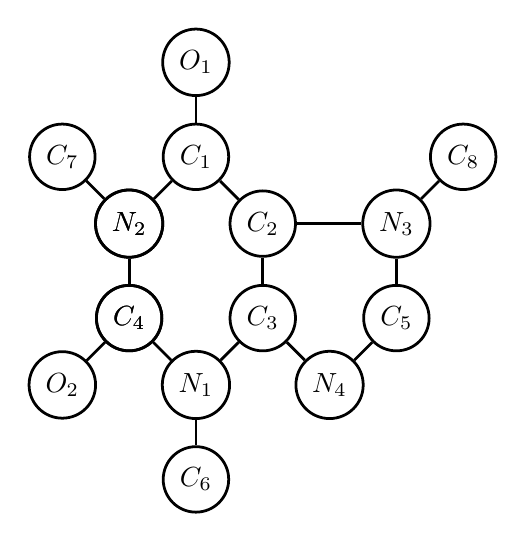
\begin{tikzpicture}[node distance={12mm}, line width=1pt, main/.style = {draw, circle}] 
\node[main] (1) []{$C_1$}; 
\node[main] (2) [below right of=1]{$C_2$}; 
\node[main] (3) [below of=2]{$C_3$}; 
\node[main] (4) [below left of=3]{$N_1$}; 
\node[main] (5) [above left of=4]{$C_4$}; 
\node[main] (6) [above of=5]{$N_2$};
\node[main] (9) [below right of=3]{$N_4$}; 
\node[main] (8) [above right of=9]{$C_5$}; 
\node[main] (7) [above of=8]{$N_3$}; 
\node[main] (10) [above of=1]{$O_1$}; 
\node[main] (11) [above left of=4]{$C_4$}; 
\node[main] (12) [above of=5]{$N_2$}; 

\node[main] (13) [below of=4]{$C_6$};  

\node[main] (17) [below left of=5]{$O_2$};

\node[main] (18) [above left of=6]{$C_7$}; 

\node[main] (22) [above right of=7]{$C_8$}; 



\draw [] (1) -- (2); 
\draw [] (2) -- (3); 
\draw [] (3) -- (4); 
\draw [] (4) -- (5); 
\draw [] (5) -- (6); 
\draw [] (6) -- (1); 
\draw [] (2) -- (7); 
\draw [] (7) -- (8); 
\draw [] (8) -- (9); 
\draw [] (9) -- (3); 
\draw [] (1) -- (10); 

\draw [] (4) -- (13); 

\draw [] (5) -- (17); 

\draw [] (6) -- (18); 

\draw [] (7) -- (22); 
\end{tikzpicture}
% \end{center}
}}
		\qquad
		\qquad
		\qquad
		\qquad
		\subfloat[][Tree decomposition]{\resizebox{0.3\textwidth}{!}{% \begin{center}
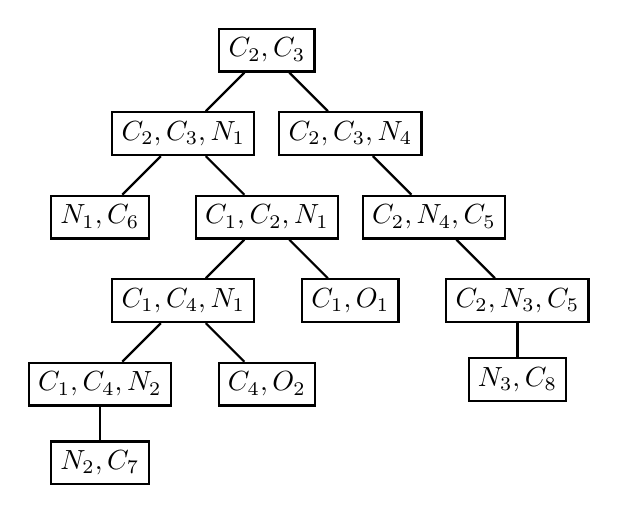
\begin{tikzpicture}[node distance={15mm}, thick, main/.style = {draw, rectangle}] 
\node[main] (0) []{$C_2,C_3$}; 
\node[main] (00) [below left of =0]{$C_2,C_3,N_1$};
\node[main] (000) [below left of =00]{$N_1,C_6$};
\node[main] (001) [below right of =00]{$C_1,C_2,N_1$};
\node[main] (0011) [below right of =001]{$C_1,O_1$};
\node[main] (0010) [below left of =001]{$C_1,C_4,N_1$};
\node[main] (00101) [below right of =0010]{$C_4,O_2$};
\node[main] (00100) [below left of =0010]{$C_1,C_4,N_2$};
\node[main] (001000) [below of =00100,,node distance={10mm}]{$N_2,C_7$};
\node[main] (01) [below right of =0]{$C_2,C_3,N_4$};
\node[main] (011) [below right of =01]{$C_2,N_4,C_5$};
\node[main] (0111) [below right of =011]{$C_2,N_3,C_5$};
\node[main] (01110) [below of =0111,,node distance={10mm}]{$N_3,C_8$};

\draw [] (0) -- (00); 
\draw [] (00) -- (000); 
\draw [] (00) -- (001); 
\draw [] (001) -- (0010); 
\draw [] (001) -- (0011); 
\draw [] (0010) -- (00100); 
\draw [] (00100) -- (001000);  
\draw [] (0010) -- (00101); 

\draw [] (0) -- (01); 
\draw [] (01) -- (011); 
\draw [] (011) -- (0111); 
\draw [] (0111) -- (01110); 

\end{tikzpicture}
% \end{center}}}
		\caption{Graph representation and tree decomposition of Caffeine.}
		\label{fig:tree_dec_caffeine}
	\end{figure}


\end{example}
% \begin{figure}[H]
% 	\centering
% 	\chemfig{=^[:270](-[:330]=^[:30]-[:90]=^[:150]-[:210])-[:210]=_[:270](%
-[:330]=_[:30]-[:330]=_[:270]-[:210]=_[:150]-[:90])-[:210](-[:270]=_[:330]%
-[:270]=_[:210]-[:150]=_[:90]-[:30])=_[:150](-[:210]=_[:270]-[:210]=_[:150]%
-[:90]=_[:30]-[:330])-[:90](-[:150]=^[:90]-[:150]=^[:210]-[:270]=^[:330]%
-[:30])=_[:30](-[:330])-[:90]=^[:30]-[:90]=^[:150]-[:210]=^[:270](-[:330])}

% 	\caption{1,2,3,4,5,6-hexakis-phenylbenzene}
% 	\label{fig:tw_2 example}
% \end{figure}


\subsection{Technical Lemmas}
\noindent We now present two technical lemmas that are crucial for development of algorithms in Section \ref{sec:algos}. These lemmas are consequences of separation properties of the tree decomposition.

\begin{lemma}\label{intseplemma}
	If $X_b$ is an introduce nodes, $X_b = X_c \cup \{v\}$, then $N(v)\cap G_b^\downarrow \subseteq X_c$.
\end{lemma}
\begin{proof} 
Let $T^\prime$ be a subtree of the tree $T$ rooted at $b$. Observe that the corresponding tree decomposition
$\mathcal{T}^\prime = \{T^\prime, \{X_t\}_{t\in V(T^\prime)}\}$ is a tree decomposition of $G_b^\downarrow$. Notice that by Definition \ref{def:tree_dec}, $T^\prime_v$ forms an induced subtree of the $T^\prime$. As $v \notin X_c$ and $c$ is the only vertex in the open neighbourhood of $b$, this implies that $T^\prime_v = \{b\}$.

Let $u$ be a vertex in $N(v) \cap G_b^\downarrow$, then by Definition \ref{def:tree_dec}, if there is an edge $uv$ in $G_b^\downarrow$, then there exists a bag containing both $u$ and $v$. But, as we have just shown that the only bag containing $v$ is $X_b$. As $u$ is a vertex in $N(v)$, this implies that $u \in X_c$.
\end{proof}
\begin{lemma}\label{joinseplemma}
	If $X_b$ is a join node with two children $X_b = X_{c_1} = X_{c_2}$, then in $G_b^\downarrow$ there is no edge between $V(G_{c_1}^\downarrow) \setminus X_b$ and $V(G_{c_2}^\downarrow) \setminus X_b$.
\end{lemma}
\begin{proof}
Let $T^\prime, T^{\prime\prime}, T^{\prime\prime\prime}$ be the subtrees of $T$ rooted at $b, c_1, c_2$ respectively. Let 
$\mathcal{T}^\prime, \mathcal{T}^{\prime\prime}, \mathcal{T}^{\prime\prime\prime}$ be the corresponding tree decompositions. We will prove the given statement by contradiction. Therefore, let us assume that $u \in V(G_{c_1}^\downarrow) \setminus X_b$, $v \in V(G_{c_2}^\downarrow) \setminus X_b$, and $uv \in E(G_b^\downarrow)$.

As $\mathcal{T}^{\prime}$ is a tree decomposition of $G^\downarrow_b$, there exists at least one bag $X_t$, such that $t \in \mathcal{T}^{\prime}$ and $u,v \in X_t$. From our initial assumption, we know that $u, v \notin X_b$, this implies that $t \neq b$. Therefore, either $t \in T^{\prime\prime}$ or $t \in T^{\prime\prime\prime}$. Without loss of generality, let us assume that $t \in T^{\prime\prime}$. As $v \in V(G_{c_2}^\downarrow) \setminus X_b$, there exists at least one bag $X_s$ such that, $ s \in T^{\prime\prime\prime}$ and $v \in X_s$. Observe that $v$ appears in both bags $X_s$ and $X_t$. Now by Definition \ref{def:tree_dec}, we know that $T^\prime_{v}$ is a connected subtree and any path connecting $s$ and $t$ goes through $b$. This implies that $X_b \in T^\prime_v$ and $v \in X_b$. This contradicts our initial assumption that $v \notin X_b$, hence completes the proof.
\end{proof}
 
\section{Our Algorithms}\label{sec:algos} 
\subsection{Counting Perfect Matchings}\label{sec:perfect_matchings}
Enumeration of Kekulé structures in organic molecules is equivalent to finding total number of perfect matchings for the underlying chemical graph of the molecule.

We present parametrized algorithms for the cases when the underlying chemical graph have bounded pathwidth and bounded treewidth respectively.



\subsubsection{Bounded Pathwidth}\label{subsec:perfect_pathwidth}
We will use a dynamic programming approach over the nice path decomposition of the given graph $G$. First we will define the dynamic programming state as follows:

\begin{definition}[Respectful Perfect Matchings]\label{def:respectful_perfect_matching}
Let us fix a nice path decomposition $\mathcal{P} = \{X_1, \dots X_r\}$ for the given graph $G$. For each $b \in [r]$ and each $M \subseteq X_b$, we define $\RP(b,M)$ as the set of all perfect matchings $F$ in a $G_b^\downarrow \setminus M$ such that each matching edge $uv \in F$ has at least one point in $G_b^\downarrow \setminus X_b$: $u \notin X_b$ or $v \notin X_b$.
\end{definition}
\begin{definition}[Dynamic Programming State for Perfect Matchings]\label{def:dp_perfect_matching}
Let us fix a nice path decomposition $\mathcal{P} = \{X_1, \dots X_r\}$ for the given graph $G$. For each $b \in [r]$ and each $M \subseteq X_b$, we define $\pma[b, M]$ to be the number of elements in the set $\RP(b,M)$.
\end{definition}

\begin{remark}
Notice that if $X_r = \varnothing$ is the root node, then $G_{r}^\downarrow = G$, and perfect matchings of $G$ are in one-to-one correspondence with respectful perfect matchings $\RP(r,\varnothing)$, which implies $\pma [r, \varnothing]$ is the total number of perfect matchings of $G$.
% If $X_l = \varnothing$ is a leaf bag, only $(X_l, \varnothing)$-respectful matching is an empty 
% matching, which means: 
% \[
% \dpt[X_l, \varnothing] = 1.
% \]
\end{remark}

We now provide a bottom-up approach for filling up the dynamic table. The dynamic table relations depend on the type of the bag. We need to consider three cases when $X_b$ is: leaf node, introduce node and forget node respectively. We refer the reader to follow proof along with Example \ref{example:explaining_dp_perfect_matchings} for better clarity of the dynamic programming approach.


\begin{itemize}
\item \textbf{Leaf node:} If $X_l$ is a leaf bag then $\RP(b,M)$ contains only empty matching as $X_l = \varnothing$. Therefore, $\pma[l,\varnothing] = 1$.
\item \textbf{Introduce node:} Let $X_b$ be an introduce bag such that $X_b = X_c \cup \{v\}$. Then the dynamic programming state corresponding to $(b,M)$ satisfies the following recurrence relations: 
\[
\pma [b,M] =
\begin{cases}
\pma [c,M\setminus v], &v \in M,\\
0, &v \not\in M.
\end{cases}
\]
In order to derive the above recurrence relations, we have to consider two possibilities for $v$.
\begin{enumerate}
\item If $v \in M$, then by Definition \ref{def:respectful_perfect_matching}, all the elements of the set $\RP(b,M)$ are in one-to-one correspondence with all the elements of the set $\RP(c, M \setminus v)$. 
\item If $v \notin M$, then for every matching $F \in \RP(b,M)$, $v$ should be covered by some edge $vw \in F$. By Lemma \ref{intseplemma}, $w \in X_{c} \subset X_b$, which contradicts the Definition \ref{def:respectful_perfect_matching}. Therefore, $\pma[b,m] = 0$ for this case, as there are no matchings satisfying the given conditions.
\end{enumerate}
This transition from $X_c$ to $X_b$ can be computed in $\bigO(1)$ time. 
\item \textbf{Forget node:} Let $X_b$ be the forget node such that $X_b = X_c \setminus \{v\}$. Then the dynamic programming state corresponding to $(b,M)$ satisfies the following recurrence relation: 

\[
\pma[b,M]=
	\pma[c, M] + \sum_{u \in X_b\setminus M:\ uv\in E(G)}\pma[c, M \cup \{v,u\}]
\]
In order to derive the above recurrence relation, let $F$ be a matching from the set $\RP(b,M)$. Note that $v \notin M$, as $M \subseteq X_b$. Therefore, $v$ will be matched by some edge $uv \in F$. Now there are two possible cases i.e., either $u \notin X_b$ or $u \in X_b$. For the former case when $u \notin X_b$, it is clear that there is a bijection between all such matchings $F$ and all elements of $\RP(c,M)$. Therefore, number of such matchings correspond to the first term $\pma[c,M]$ of the recurrence relation. Now let's consider the latter case when $u \in X_b$, then the matching $F \setminus uv \in \RP(c,M M \cup \{u, v\})$, and number of such matchings correspond to the second term $\sum_{u \in X_b\setminus M:\ uv\in E(G)}\pma[c, M \cup \{v,u\}]$ of the recurrence relation.





% To prove that consider any $(X_b, M)$-respectful matching $F$. Since $v \notin M$, $v$ should be matched with some point, say, $u$. Then if $u\notin X_b$, matching $F$ is $(X_{c}, M)$-respectful, and number of such cases corresponds to the first term. If $u \in X_b$ then mathching $F \setminus uv$ is $(X_{c}, M \cup \{u, v\})$ respectful and correspondence is one-to-one.  

This transition to $X_b$ can be computed in $\bigO(\lvert X_b\rvert) = \bigO(\pw(G))$ time.
\end{itemize}


\begin{proposition}\label{prop:comp_pw_perfmat}
The time complexity for finding the total number of perfect matchings for a graph $G = (V,E)$, with $\lvert V \rvert = n$ and pathwidth $\pw$, using the above algorithm is $\bigO(n\cdot \poly(\pw) \cdot2^{\pw})$.
% The final complexity is $\bigO(n\cdot \textup{pw}\cdot2^{\textup{pw}})$
\end{proposition}
\begin{proof}
For each bag, we have at most $2^{\pw}$ dynamic programming states, and for each state we spend at most $\bigO(\poly(\pw))$ time. It is known that there are at most $\bigO(n \cdot \pw)$ bags for any nice path decomposition of $G$ \cite[Chapter 7]{cygan2015parameterized}. Therefore, we spend at most $\bigO(n\cdot \poly(\pw) \cdot2^{\pw})$ time to completely fill the dymamic programming table.
\end{proof}
\subsubsection{Bounded Treewidth}\label{subsec:perfect_treewidth}
We will use a dynamic programming approach over the nice tree decomposition of the given graph $G$. The definitions of respectful perfect matchings and dynamic programming states used here are same as Section \ref{subsec:perfect_pathwidth}. Let $\mathcal{T} = \{T, \{X_t\}_{t \in V(T)}\}$ be a nice tree decomposition of the graph $G = (V,E)$ under consideration.

% We will use a dynamic programming over the nice tree decomposition. Definitions of dynamic programming and respectfulness have only cosmetic differences with path decomposition case. Let us fix a nice tree decomposition $\mathcal{T} = \{T, \{X_t\}_{t \in V(T)}\}$. For each $b \in T$ and each $M \subseteq X_b$ we will define $\dpt[b, M]$ as a number of perfect matchings in a $G_b^\downarrow \setminus M$ such that each matching edge $uv$ has at least on point in $G_b^\downarrow \setminus X_b$: $u \notin X_b$ or $v \notin X_b$. We call such matchings \textit{respectful} to the $(X_b, M)$.


% \begin{remark}

% \end{remark}
% If $X_l = \varnothing$ is a leaf bag, we have only empty $(X_l, \varnothing)$-respectful matching, which means 
% \[
% 	\dpt[X_l, \varnothing] = 1.
% \]

% Also for the root bag $X_r$, $\dpt[X_r, \varnothing]$ contains number of perfect matchings in a whole graph $G$.


% Cases of introduce and forget nodes repet verbatim. We need only consider merge case now. 
We now provide a bottom-up approach for filling up the dynamic table. The dynamic table relations depend on the type of the bag. There are four possible cases for the type of bags, i.e., when $X_b$ is: leaf node, introduce node, forget node and join node respectively. The reccurrence relations for leaf node, introduce node and forget node remains the same as Section \ref{subsec:perfect_pathwidth}. Therefore, we only need to consider the case of join node which is described as follows:
\begin{itemize}
	\item \textbf{Join node:} Let $X_b$ be the join node with $X_{c_1}$ and $X_{c_2}$ as its children. Then the dynamic programming state corresponding to $(b,M)$ will satisfy the following recurrence relation:
\[
\pma[b,M] = \sum_{H_1 \sqcup H_2 = X_b \setminus M}\pma[c_1,M\cup H_2]\cdot \pma[c_2, M\cup H_1]
% \\
% &=\sum_{H \subseteq X_b \setminus M}\pma[c_1,M\cup H]\cdot \pma[c_2, X_b \setminus H],\\
\]

where $H_1 \sqcup H_2 = X_b \setminus M$ means $H_1 \cup H_2 = X_b \setminus M$ and $H_1 \cap H_2 = \varnothing$. 
% This two formulas yields same result, but first easier to analyze and second easier to implement.  
In order to derive the above recurrence relation, let $F$ be a matching from the set $\RP(b,M)$. By Lemma \ref{joinseplemma}, $F$ doesn't have any edges between $G_{c_1}^\downarrow \setminus X_b$ and $G_{c_2}^\downarrow \setminus X_b$. Therefore, it can be split into two matchings, $F_1 := E(G_{c_1}^\downarrow) \cap F$ and $F_2 := E(G_{c_2}^\downarrow) \cap F$. Let $H_1 := V(F_1) \cap X_b$ and $H_2 := V(F_2) \cap X_b$. It is clear from the Definition \ref{def:respectful_perfect_matching}, that $F_1 \in \RP(c_1,M \cup H_2)$ and $F_2 \in \RP(c_2,M \cup H_1)$. If we choose $H_1$ and $H_2$ such that $H_1 \sqcup H_2 = X_b \setminus M$, then for all such matchings $F_1 \in \RP(c_1,M\cup H_2)$ and $F_2 \in \RP(c_2, M\cup H_1)$, we get a matching $ F = F_1 \cup F_2$, such that $F \in \RP(b,M)$. This leads to our recurrence relation.



% Consider arbitrary $(X_b, M)$-respectful matching $F$. By lemma \ref{joinseplemma} $F$ do not have edges between $G_{c_1}^\downarrow \setminus X_b$ and $G_{c_2}^\downarrow \setminus X_b$. Let us split this matching $F$ into $F_1 := E(G_{c_1}^\downarrow) \cap F$, $F_2 := E(G_{c_2}^\downarrow) \cap F$, also let $H_1 := V(F_1) \cap X_b$, $H_2 := V(F_2) \cap X_b$. Observe that $F_1$ is $(X_{c_1}, M \cup H_2)$-respectful and $F_2$ is $(X_{c_2}, M \cup H_1)$-respectful. Notice that if $H_1, H_2$ are chosen, $F_1, F_2$ acts independently, so when $H_1, H_2$ fixed such matching could be counted as $\dpt[c_1, M \cup H_2] \cdot \dpt[c_2, M \cup H_1]$, which leads to our formula. 

\end{itemize}

\begin{proposition}\label{prop:comp_tw_perfmat}
The time complexity for finding the total number of perfect matchings for a graph $G = (V,E)$, with $\lvert V \rvert = n$ and treewidth $\twi$, using the above algorithm is $\bigO(n\cdot \poly(\twi)\cdot3^{\twi})$.
% With this, the final complexity of the algorithm increases to .
\end{proposition}
\begin{proof}
The transition for a join node is the most expensive operation for this algorithm, the rest of the cases are similar to the dynamic programming on nice path decomposition in Section \ref{subsec:perfect_pathwidth}.
Note that the recurrence relation for the dynamic programming state of join node can be rewritten as:
\[
\sum_{H \subseteq X_b \setminus M}\pma[c_1,M\cup H]\cdot \pma[c_2, X_b \setminus H]
\]

For each bag $X_b$ and for each $M \subseteq X_b$, we spend at most $\bigO(\poly(\twi)\cdot 2^{\lvert X_B \rvert - \lvert M \rvert})$ time. By using the binomial theorem, the total time spend for each bag $X_b$ for all possible subsets $M$ is $\bigO(\poly(\twi)\cdot 3^{\lvert X_B \rvert})$. It is known that there are at most $\bigO(n \cdot \twi)$ bags for any nice tree decomposition of $G$ \cite[Chapter 7]{cygan2015parameterized}. Therefore, we spend at most $\bigO(n\cdot \poly(\twi)\cdot3^{\twi})$ time to completely fill the dymamic programming table.
\end{proof}

\begin{example}\label{example:explaining_dp_perfect_matchings}
	In this example, we explain the above algorithm explicitly with figures for all cases of nodes in the tree decomposition. Red color nodes in the following figures are elements of the set $M$ defined in Definition \ref{def:respectful_perfect_matching}.

	\begin{itemize}
		\item Introduce Node:
		\begin{figure}[H]
			\centering
			\resizebox{0.6\textwidth}{!}{\begin{tikzpicture}[line width=1pt,node distance=14mm ,main/.style = {draw, rectangle},scale=1] 
    \node[scale=.8] at (0,5.5){$\textup{PerfMatch}[b,\{x_1,x_2,x_3,x_4\}]$};
   \node[main] at (0,4) (9) {
   \begin{tikzpicture}[line width=1pt,node distance=14mm ,main/.style = {draw, circle},scale=1] 
   \node[main,color=red, densely dashed] at (0,1) (x1) {\texttt{$x_1$}};
   \node[main,color=red,densely dashed] at (1,1) (x2) {\texttt{$x_2$}};
       \node[main,color=red,densely dashed] at (0,0) (x3) {\texttt{$x_3$}};
       \node[main,color=red,densely dashed] at (1,0) (x4) {\texttt{$x_4$}};
      \draw (x1) -- (x2);
       \draw (x1) -- (x3);
      \draw (x2) -- (x3);
      \draw (x3) -- (x4);
   \end{tikzpicture}
       };
   
    \node[scale=.8] at (3.5,5.5){$\textup{PerfMatch}[b,\{x_1,x_4\}]$};
       \node[main] at (3.5,4) (9) {
   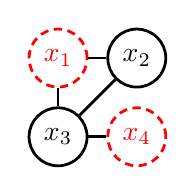
\begin{tikzpicture}[line width=1pt,node distance=14mm ,main/.style = {draw, circle},scale=1] 
   \node[main,color=red,densely dashed] at (0,1) (x1) {\texttt{$x_1$}};
   \node[main,color=black] at (1,1) (x2) {\texttt{$x_2$}};
       \node[main,color=black] at (0,0) (x3) {\texttt{$x_3$}};
       \node[main,color=red,densely dashed] at (1,0) (x4) {\texttt{$x_4$}};
      \draw (x1) -- (x2);
       \draw (x1) -- (x3);
      \draw (x2) -- (x3);
      \draw (x3) -- (x4);
   \end{tikzpicture}
       };
   
   \node[scale=.8] at (7,5.5){$\textup{PerfMatch}[b,\{x_1,x_2\}]$};
       \node[main] at (7,4) (9) {
   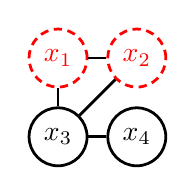
\begin{tikzpicture}[line width=1pt,node distance=14mm ,main/.style = {draw, circle},scale=1] 
   \node[main,color=red,densely dashed] at (0,1) (x1) {\texttt{$x_1$}};
   \node[main,color=red,densely dashed] at (1,1) (x2) {\texttt{$x_2$}};
       \node[main,color=black] at (0,0) (x3) {\texttt{$x_3$}};
       \node[main,color=black] at (1,0) (x4) {\texttt{$x_4$}};
      \draw (x1) -- (x2);
       \draw (x1) -- (x3);
      \draw (x2) -- (x3);
      \draw (x3) -- (x4);
   \end{tikzpicture}
       };
       
    \node[scale=.8] at (0,1.5){$\textup{PerfMatch}[c,\{x_2,x_3,x_4\}]$};
       \node[main] at (0,0) (8) {
   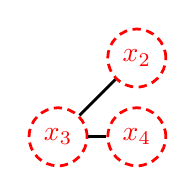
\begin{tikzpicture}[line width=1pt,node distance=14mm ,main/.style = {draw, circle},scale=1] 
   \node[main,color=red,densely dashed] at (1,1) (x2) {\texttt{$x_2$}};
       \node[main,color=red,densely dashed] at (0,0) (x3) {\texttt{$x_3$}};
       \node[main,color=red,densely dashed] at (1,0) (x4) {\texttt{$x_4$}};
      \draw (x2) -- (x3);
      \draw (x3) -- (x4);
   \end{tikzpicture}
   };
   
    \node[scale=.8] at (3.5,1.5){$\textup{PerfMatch}[c,\{x_4\}]$};
   \node[main] at (3.5,0) (8) {
   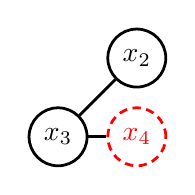
\begin{tikzpicture}[line width=1pt,node distance=14mm ,main/.style = {draw, circle},scale=1] 
   \node[main,color=black] at (1,1) (x2) {\texttt{$x_2$}};
       \node[main,color=black] at (0,0) (x3) {\texttt{$x_3$}};
       \node[main,color=red,densely dashed] at (1,0) (x4) {\texttt{$x_4$}};
      \draw (x2) -- (x3);
      \draw (x3) -- (x4);
   \end{tikzpicture}
   };
   
    \node[scale=.8] at (7,1.5){$\textup{PerfMatch}[c,\{x_2\}]$};
   \node[main] at (7,0) (8) {
   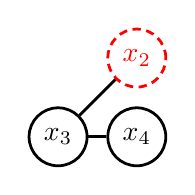
\begin{tikzpicture}[line width=1pt,node distance=14mm ,main/.style = {draw, circle},scale=1] 
   \node[main,color=red,densely dashed] at (1,1) (x2) {\texttt{$x_2$}};
       \node[main,color=black] at (0,0) (x3) {\texttt{$x_3$}};
       \node[main,color=black] at (1,0) (x4) {\texttt{$x_4$}};
      \draw (x2) -- (x3);
      \draw (x3) -- (x4);
   \end{tikzpicture}
   };
   
   
   
       \draw [->](0,2) -- (0,2.5);
       \draw [->](3.5,2) -- (3.5,2.5);
       \draw [->](7,2) -- (7,2.5);
   
   
    \node[scale=.8] at (10.5,5.5){$\textup{PerfMatch}[b,\{x_3,x_4\}]$};
       \node[main] at (10.5,4) (9) {
   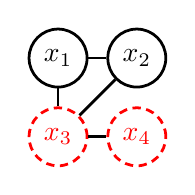
\begin{tikzpicture}[line width=1pt,node distance=14mm ,main/.style = {draw, circle},scale=1] 
   \node[main,color=black] at (0,1) (x1) {\texttt{$x_1$}};
   \node[main,color=black] at (1,1) (x2) {\texttt{$x_2$}};
       \node[main,color=red,densely dashed] at (0,0) (x3) {\texttt{$x_3$}};
       \node[main,color=red,densely dashed] at (1,0) (x4) {\texttt{$x_4$}};
      \draw (x1) -- (x2);
       \draw (x1) -- (x3);
      \draw (x2) -- (x3);
      \draw (x3) -- (x4);
   \end{tikzpicture}
       };
   
       \draw [->](10.5,1) -- (10.5,2.5);
       \node[scale=3] at (10.5,0){$\varnothing$};
       %\node[text width=6cm] at (2,-2){$\DP[i,c]$};
       %\node[text width=6cm] at (5.5,-2){$\DP[i,c+\{x_4\to \texttt{gray/dotted}]$};
      
   \end{tikzpicture}
   }
			\label{fig:introduce_node}
			\caption{Example for introduce node.}
		\end{figure}
		\item Forget Node:
		\begin{figure}[H]
			\centering
			\resizebox{0.6\textwidth}{!}{% !TEX root = ../main.tex
\begin{tikzpicture}[line width=1pt,node distance=14mm ,main/.style = {draw, rectangle},scale=1] 

    \node[scale=.8] at (3,6){$\textup{PerfMatch}[b,\{x_4\}]$};
       
       \node[main] at (3,4.5) (9) {
   \begin{tikzpicture}[line width=1pt,node distance=14mm ,main/.style = {draw, circle},scale=1] 
   \node[main,color=black] at (1,1) (x2) {\texttt{$x_2$}};
       \node[main,color=black] at (0,0) (x3) {\texttt{$x_3$}};
       \node[main,fill=red!40!white,densely dashed] at (1,0) (x4) {\texttt{$x_4$}};
      \draw (x2) -- (x3);
      \draw (x3) -- (x4);
   \end{tikzpicture}
       };
       
    \node[scale=.8] at (-1,1.5){$\textup{PerfMatch}[c,\{x_4\}]$};
       \node[main] at (-1,0) (8) {
   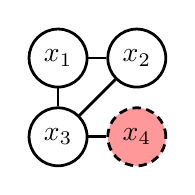
\begin{tikzpicture}[line width=1pt,node distance=14mm ,main/.style = {draw, circle},scale=1] 
   \node[main,color=black] at (0,1) (x1) {\texttt{$x_1$}};
   \node[main,color=black] at (1,1) (x2) {\texttt{$x_2$}};
       \node[main,color=black] at (0,0) (x3) {\texttt{$x_3$}};
       \node[main,fill=red!40!white,densely dashed] at (1,0) (x4) {\texttt{$x_4$}};
      \draw (x1) -- (x2);
       \draw (x1) -- (x3);
      \draw (x2) -- (x3);
      \draw (x3) -- (x4);
   \end{tikzpicture}
   };
   
    \node[scale=.8] at (3,1.5){$\textup{PerfMatch}[c,\{x_4\}\cup \{x_1,x_2\}]$};
   \node[main] at (3,0) (8) {
   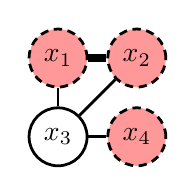
\begin{tikzpicture}[line width=1pt,node distance=14mm ,main/.style = {draw, circle},scale=1] 
   \node[main,fill=red!40!white,densely dashed] at (0,1) (x1) {\texttt{$x_1$}};
   \node[main,fill=red!40!white,densely dashed] at (1,1) (x2) {\texttt{$x_2$}};
       \node[main,color=black] at (0,0) (x3) {\texttt{$x_3$}};
       \node[main,fill=red!40!white,densely dashed] at (1,0) (x4) {\texttt{$x_4$}};
      \draw [line width = 3pt, color=black]  (x1) -- (x2);
       \draw (x1) -- (x3);
      \draw (x2) -- (x3);
      \draw (x3) -- (x4);
   \end{tikzpicture}
   };
   
    \node[scale=.8] at (7,1.5){$\textup{PerfMatch}[c,\{x_4\}\cup \{x_1,x_3\}]$};
   \node[main] at (7,0) (8) {
   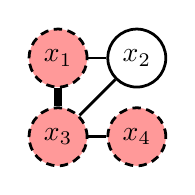
\begin{tikzpicture}[line width=1pt,node distance=14mm ,main/.style = {draw, circle},scale=1] 
   \node[main,fill=red!40!white,densely dashed] at (0,1) (x1) {\texttt{$x_1$}};
   \node[main,color=black] at (1,1) (x2) {\texttt{$x_2$}};
       \node[main,fill=red!40!white,densely dashed] at (0,0) (x3) {\texttt{$x_3$}};
       \node[main,fill=red!40!white,densely dashed] at (1,0) (x4) {\texttt{$x_4$}};
      \draw (x1) -- (x2);
       \draw [line width = 3pt, color=black] (x1) -- (x3);
      \draw (x2) -- (x3);
      \draw (x3) -- (x4);
   \end{tikzpicture}
   };
   
       \draw [decorate,decoration={brace,amplitude=10}] (0,2.5) -- (6,2.5) node [black,midway,xshift=-0.6cm] {};
   
       %\node[text width=6cm] at (2,-2){$\DP[i,c]$};
       %\node[text width=6cm] at (5.5,-2){$\DP[i,c+\{x_4\to \texttt{gray/dotted}]$};
      
   \end{tikzpicture}
   }
			\label{fig:forget_node}
			\caption{Example for forget node.}
		\end{figure}
		\item Join Node:
		\begin{figure}[H]
			\centering
			\resizebox{0.6\textwidth}{!}{% !TEX root = ../main.tex
\begin{tikzpicture}[line width=1pt,node distance=14mm ,main/.style = {draw, rectangle},scale=1] 

    \node[scale=.8] at (-4,1){$\textup{PerfMatch}[b,\{x_1,x_4\}]$};
       \node[main] at (-4,-0.5) (9) {
   \begin{tikzpicture}[line width=1pt,node distance=14mm ,main/.style = {draw, circle},scale=1] 
   \node[main,fill=red!40!white,densely dashed] at (0,1) (x1) {\texttt{$x_1$}};
   \node[main,color=black] at (1,1) (x2) {\texttt{$x_2$}};
       \node[main,color=black] at (0,0) (x3) {\texttt{$x_3$}};
       \node[main,fill=red!40!white,densely dashed] at (1,0) (x4) {\texttt{$x_4$}};
      \draw  (x1) -- (x2);
       \draw (x1) -- (x3);
      \draw (x2) -- (x3);
      \draw (x3) -- (x4);
   \end{tikzpicture}
       };
       
    \node[scale=.8] at (0,5.5){$\textup{PerfMatch}[c_1,\{x_1,x_4\}\cup \{x_2,x_3\}]$};
       \node[main] at (0,4) (8) {
   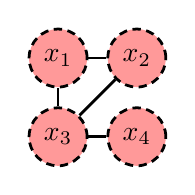
\begin{tikzpicture}[line width=1pt,node distance=14mm ,main/.style = {draw, circle},scale=1] 
   \node[main,fill=red!40!white,densely dashed] at (0,1) (x1) {\texttt{$x_1$}};
   \node[main,fill=red!40!white,densely dashed] at (1,1) (x2) {\texttt{$x_2$}};
       \node[main,fill=red!40!white,densely dashed] at (0,0) (x3) {\texttt{$x_3$}};
       \node[main,fill=red!40!white,densely dashed] at (1,0) (x4) {\texttt{$x_4$}};
      \draw (x1) -- (x2);
       \draw (x1) -- (x3);
      \draw (x2) -- (x3);
      \draw (x3) -- (x4);
   \end{tikzpicture}
   };
   
    \node[scale=3] at (2,4){$\cdot$};
   
    \node[scale=.8] at (4,5.5){$\textup{PerfMatch}[c_2,\{x_1,x_4\}\cup \{\}]$};
   \node[main] at (4,4) (8) {
   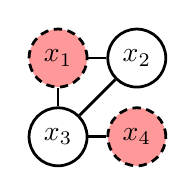
\begin{tikzpicture}[line width=1pt,node distance=14mm ,main/.style = {draw, circle},scale=1] 
   \node[main,fill=red!40!white,densely dashed] at (0,1) (x1) {\texttt{$x_1$}};
   \node[main,color=black] at (1,1) (x2) {\texttt{$x_2$}};
       \node[main,color=black] at (0,0) (x3) {\texttt{$x_3$}};
       \node[main,fill=red!40!white,densely dashed] at (1,0) (x4) {\texttt{$x_4$}};
      \draw (x1) -- (x2);
       \draw (x1) -- (x3);
      \draw (x2) -- (x3);
      \draw (x3) -- (x4);
   \end{tikzpicture}
   };
   
    \node[scale=.8] at (0,2.5){$\textup{PerfMatch}[c_1,\{x_1,x_4\}\cup \{x_3\}]$};
   \node[main] at (0,1) (8) {
   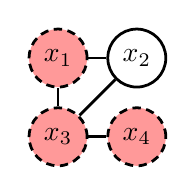
\begin{tikzpicture}[line width=1pt,node distance=14mm ,main/.style = {draw, circle},scale=1] 
   \node[main,fill=red!40!white,densely dashed] at (0,1) (x1) {\texttt{$x_1$}};
   \node[main,color=black] at (1,1) (x2) {\texttt{$x_2$}};
       \node[main,fill=red!40!white,densely dashed] at (0,0) (x3) {\texttt{$x_3$}};
       \node[main,fill=red!40!white,densely dashed] at (1,0) (x4) {\texttt{$x_4$}};
      \draw (x1) -- (x2);
       \draw (x1) -- (x3);
      \draw (x2) -- (x3);
      \draw (x3) -- (x4);
   \end{tikzpicture}
   };
   
    \node[scale=3] at (2,1){$\cdot$};
   
    \node[scale=.8] at (4,2.5){$\textup{PerfMatch}[c_2,\{x_1,x_4\}\cup \{x_2\}]$};
   \node[main] at (4,1) (8) {
   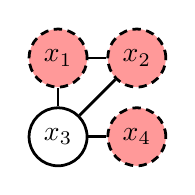
\begin{tikzpicture}[line width=1pt,node distance=14mm ,main/.style = {draw, circle},scale=1] 
   \node[main,fill=red!40!white,densely dashed] at (0,1) (x1) {\texttt{$x_1$}};
   \node[main,fill=red!40!white,densely dashed] at (1,1) (x2) {\texttt{$x_2$}};
       \node[main,color=black] at (0,0) (x3) {\texttt{$x_3$}};
       \node[main,fill=red!40!white,densely dashed] at (1,0) (x4) {\texttt{$x_4$}};
      \draw (x1) -- (x2);
       \draw (x1) -- (x3);
      \draw (x2) -- (x3);
      \draw (x3) -- (x4);
   \end{tikzpicture}
   };
   
    \node[scale=.8] at (0,-0.5){$\textup{PerfMatch}[c_1,\{x_1,x_4\}\cup \{x_2\}]$};
   \node[main] at (0,-2) (8) {
   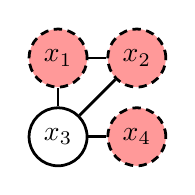
\begin{tikzpicture}[line width=1pt,node distance=14mm ,main/.style = {draw, circle},scale=1] 
   \node[main,fill=red!40!white,densely dashed] at (0,1) (x1) {\texttt{$x_1$}};
   \node[main,fill=red!40!white,densely dashed] at (1,1) (x2) {\texttt{$x_2$}};
       \node[main,color=black] at (0,0) (x3) {\texttt{$x_3$}};
       \node[main,fill=red!40!white,densely dashed] at (1,0) (x4) {\texttt{$x_4$}};
      \draw (x1) -- (x2);
       \draw (x1) -- (x3);
      \draw (x2) -- (x3);
      \draw (x3) -- (x4);
   \end{tikzpicture}
   };
   
    \node[scale=3] at (2,-2){$\cdot$};
   
    \node[scale=.8] at (4,-0.5){$\textup{PerfMatch}[c_2,\{x_1,x_4\}\cup \{x_3\}]$};
   \node[main] at (4,-2) (8) {
   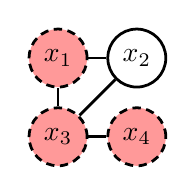
\begin{tikzpicture}[line width=1pt,node distance=14mm ,main/.style = {draw, circle},scale=1] 
   \node[main,fill=red!40!white,densely dashed] at (0,1) (x1) {\texttt{$x_1$}};
   \node[main,color=black] at (1,1) (x2) {\texttt{$x_2$}};
       \node[main,fill=red!40!white,densely dashed] at (0,0) (x3) {\texttt{$x_3$}};
       \node[main,fill=red!40!white,densely dashed] at (1,0) (x4) {\texttt{$x_4$}};
      \draw (x1) -- (x2);
       \draw (x1) -- (x3);
      \draw (x2) -- (x3);
      \draw (x3) -- (x4);
   \end{tikzpicture}
   };
   
    \node[scale=.8] at (0,-3.5){$\textup{PerfMatch}[c_1,\{x_1,x_4\}\cup \{\}]$};
   \node[main] at (0,-5) (8) {
   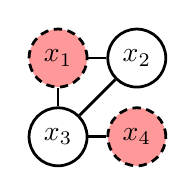
\begin{tikzpicture}[line width=1pt,node distance=14mm ,main/.style = {draw, circle},scale=1] 
   \node[main,fill=red!40!white,densely dashed] at (0,1) (x1) {\texttt{$x_1$}};
   \node[main,color=black] at (1,1) (x2) {\texttt{$x_2$}};
       \node[main,color=black] at (0,0) (x3) {\texttt{$x_3$}};
       \node[main,fill=red!40!white,densely dashed] at (1,0) (x4) {\texttt{$x_4$}};
      \draw (x1) -- (x2);
       \draw (x1) -- (x3);
      \draw (x2) -- (x3);
      \draw (x3) -- (x4);
   \end{tikzpicture}
   };
   
    \node[scale=3] at (2,-5){$\cdot$};
   
     \node[scale=.8] at (4,-3.5){$\textup{PerfMatch}[c_2,\{x_1,x_4\}\cup \{x_2,x_3\}]$};
   \node[main] at (4,-5) (8) {
   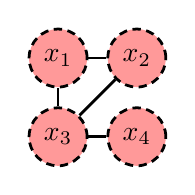
\begin{tikzpicture}[line width=1pt,node distance=14mm ,main/.style = {draw, circle},scale=1] 
   \node[main,fill=red!40!white,densely dashed] at (0,1) (x1) {\texttt{$x_1$}};
   \node[main,fill=red!40!white,densely dashed] at (1,1) (x2) {\texttt{$x_2$}};
       \node[main,fill=red!40!white,densely dashed] at (0,0) (x3) {\texttt{$x_3$}};
       \node[main,fill=red!40!white,densely dashed] at (1,0) (x4) {\texttt{$x_4$}};
      \draw (x1) -- (x2);
       \draw (x1) -- (x3);
      \draw (x2) -- (x3);
      \draw (x3) -- (x4);
   \end{tikzpicture}
   };
   
       \draw [decorate,decoration={brace,amplitude=10}] (-2,-5) -- (-2,4) node [black,midway,xshift=-0.6cm] {};
   
       %\draw [->](-2,3.5) -- (-3,2.5);
       %\draw [->](-2,1) -- (-3,0.5);
       %\draw [->](-2,-2) -- (-3,-1.5);
       %\draw [->](-2,-4.5) -- (-3,-3.5);
       %\draw [->](3.5,-2.5) -- (5,-3);
       %\draw [->](3.5,-5) -- (5,-4.5);
       %\draw [->](3.5,-7.5) -- (5,-6);
       %\node[text width=6cm] at (2,-2){$\DP[i,c]$};
       %\node[text width=6cm] at (5.5,-2){$\DP[i,c+\{x_4\to \texttt{gray/dotted}]$};
      
   \end{tikzpicture}}
			\label{fig:join_node}
			\caption{Example for join node.}
		\end{figure}
	\end{itemize}
	
\end{example}

\subsection{Counting Matchings}\label{sec:matchings}
\subsubsection{Bounded Pathwidth}\label{sec:pathwidth_matchings}
We will use a dynamic programming approach over the nice path decomposition of the given graph $G$. First we will define the dynamic programming state as follows:

\begin{definition}[Respectful Matchings]\label{def:respectful_matching}
Let us fix a nice path decomposition $\mathcal{P} = \{X_1, \dots X_r\}$ for the given graph $G$. For each $b \in [r]$ and each $M \subseteq X_b$, we define $\RM(b,M)$ as the set of all matchings $F$ in a $G_b^\downarrow \setminus M$ such that each matching edge $uv \in F$ has at least one point in $G_b^\downarrow \setminus X_b$: $u \notin X_b$ or $v \notin X_b$ and each point from $X_b \setminus M$ is covered by $F$.
\end{definition}
\begin{definition}[Dynamic Programming State for Matchings]\label{def:dp_matching}
Let us fix a nice path decomposition $\mathcal{P} = \{X_1, \dots X_r\}$ for the given graph $G$. For each $b \in [r]$ and each $M \subseteq X_b$, we define $\ma[b, M]$ to be the number of elements in the set $\RM(b,M)$.
\end{definition}

\begin{remark}
Notice that if $X_r = \varnothing$ is the root node, then $G_{r}^\downarrow = G$, and all matchings of $G$ are in one-to-one correspondence with respectful matchings $\RM(r,\varnothing)$, which implies $\ma [r, \varnothing]$ is the total number of matchings of $G$.
% If $X_l = \varnothing$ is a leaf bag, only $(X_l, \varnothing)$-respectful matching is an empty 
% matching, which means: 
% \[
% \dpt[X_l, \varnothing] = 1.
% \]
\end{remark}

We now provide a bottom-up approach for filling up the dynamic table. The dynamic table relations depend on the type of the bag. We need to consider three cases when $X_b$ is: leaf node, introduce node and forget node respectively.


\begin{itemize}
\item \textbf{Leaf node:} If $X_l$ is a leaf bag then $\RM(b,M)$ contains only empty matching as $X_l = \varnothing$. Therefore, $\ma[l,\varnothing] = 1$.
\item \textbf{Introduce node:} Let $X_b$ be the introduce bag such that $X_b = X_c \cup \{v\}$. Then the dynamic programming state corresponding to $(b,M)$ satisfies the following recurrence relations: 
\[
\ma [b,M] =
\begin{cases}
\ma [c,M\setminus v], &v \in M,\\
0, &v \not\in M.
\end{cases}
\]
In order to derive the above recurrence relations, we have to consider two possibilities for $v$.
\begin{enumerate}
\item If $v \in M$, then by Definition \ref{def:respectful_matching}, all the elements of the set $\RM(b,M)$ are in one-to-one correspondence with all the elements of the set $\RM(c, M \setminus v)$. 
\item If $v \notin M$, then for every matching $F \in \RP(b,M)$, $v$ should be covered by some edge $vw \in F$. By Lemma \ref{intseplemma}, $w \in X_{c} \subset X_b$, which contradicts the Definition \ref{def:respectful_matching}. Therefore, $\ma[b,m] = 0$ for this case, as there are no matchings satisfying the given conditions.
\end{enumerate}
This transition from $X_c$ to $X_b$ can be computed in $\bigO(1)$ time. 
\item \textbf{Forget node:} Let $X_b$ be the forget node such that $X_b = X_c \setminus \{v\}$. Then the dynamic programming state corresponding to $(b,M)$ satisfies the following recurrence relation: 

% \[
% \pma[b,M]=
% 	\pma[c, M] + \sum_{u \in X_b\setminus M:\ uv\in E(G)}\pma[c, M \cup \{v,u\}].
% \]

\begin{align*} 
\ma[b,M]= \ma[c, M] &+  \ma[c, M \cup \{v\}] \\
&+ \sum_{u \in X_b\setminus M:\ uv\in E(G)}\ma[c, M \cup \{v,u\}]
\end{align*}
% \[
% \ma[b,M]=
% \ma[c, M] + \ma[c, M \cup \{v\}] + \sum_{u \in X_b\setminus M:\ uv\in E(G)}\ma[c, M \cup \{v,u\}]
% \]
In order to derive the above recurrence relation, let $F$ be a matching from the set $\RM(b,M)$. Note that $v \notin M$, as $M \subseteq X_b$. There are two possibilities for $v$ i.e., either it will be covered by some edge in $F$ or it remains unmatched. For the latter case, all such matchings $F$ for which $v$ remains unmatched are in one-to-one correpondence with all matchings of the set $\RM(c,M\cup\{v\}$, and number of such matchings correspond to the second term $\ma[c, M \cup \{v\}]$ of the recurrsion. Now let us consider the second case, where $v$ will be matched by some edge $uv \in F$. Now there are again two possible cases to consider i.e., either $u \notin X_b$ or $u \in X_b$. For the former case when $u \notin X_b$, it is clear that there is a bijection between all such matchings $F$ and all elements of $\RM(c,M)$. Therefore, number of such matchings correspond to the first term $\ma[c,M]$ of the recurrence relation. Now let's consider the latter case when $u \in X_b$, then the matching $F \setminus uv \in \RM(c,M M \cup \{u, v\})$, and number of such matchings correspond to the last term $\sum_{u \in X_b\setminus M:\ uv\in E(G)}\ma[c, M \cup \{v,u\}]$ of the recurrence relation.


% To prove that consider any $(X_b, M)$-respectful matching $F$. If $v$ unmached, $v \notin V(F)$ and $F$ is $(X_c, M \cup \{v\})$-respectful. If $v$ is matched with some vertex $u$, we have two cases:  either $w \notin X_b$ $w \in X_b$. In a first case the mathching $F$ is $(X_c, M)$-respectful, and this case corresponds to the term $\dpt[c, M \cup \{v\}]$. If $w \in X_b$, then exist edge $uv$ and matching $F \setminus uv$ is $(X_c, M \cup \{v, u\})$-respectful, which corresponds to the sum of $\dpt[c, M\cup \{v, u\}]$ terms. All correspondences is one-to-one.  


% To prove that consider any $(X_b, M)$-respectful matching $F$. Since $v \notin M$, $v$ should be matched with some point, say, $u$. Then if $u\notin X_b$, matching $F$ is $(X_{c}, M)$-respectful, and number of such cases corresponds to the first term. If $u \in X_b$ then mathching $F \setminus uv$ is $(X_{c}, M \cup \{u, v\})$ respectful and correspondence is one-to-one.  

This transition to $X_b$ can be computed in $\bigO(\lvert X_b\rvert) = \bigO(\pw(G))$ time.
\end{itemize}


\begin{proposition}\label{prop:comp_pw_mat}
The time complexity for finding the total number of matchings for a graph $G = (V,E)$, with $\lvert V \rvert = n$ and pathwidth $\pw$, using the above algorithm is $\bigO(n\cdot \poly(\pw) \cdot2^{\pw})$.
% The final complexity is $\bigO(n\cdot \textup{pw}\cdot2^{\textup{pw}})$
\end{proposition}
\begin{proof}
Same proof as Proposition \ref{prop:comp_pw_perfmat}.
% For each bag, we have atmost $2^{\pw}$ dynamic programming states, and for each state we spend atmost $\bigO(\poly(\pw))$ time. It is known that there are atmost $\bigO(n)$ bags for any nice path decomposition of $G$ \cite[Chapter 7]{cygan2015parameterized}. Therefore, we spend atmost $\bigO(n\cdot \poly(\pw) \cdot2^{\pw})$ time to completely fill the dymamic programming table.
\end{proof}

\subsubsection{Bounded Treewidth}\label{subsec:matching_treewidth}
We will use a dynamic programming approach over the nice tree decomposition of the given graph $G$. The definitions of respectful matchings and dynamic programming states used here are same as Section \ref{sec:pathwidth_matchings}. Let $\mathcal{T} = \{T, \{X_t\}_{t \in V(T)}\}$ be a nice tree decomposition of the graph $G = (V,E)$ under consideration.

% We will use a dynamic programming over the nice tree decomposition. Definitions of dynamic programming and respectfulness have only cosmetic differences with path decomposition case. Let us fix a nice tree decomposition $\mathcal{T} = \{T, \{X_t\}_{t \in V(T)}\}$. For each $b \in T$ and each $M \subseteq X_b$ we will define $\dpt[b, M]$ as a number of perfect matchings in a $G_b^\downarrow \setminus M$ such that each matching edge $uv$ has at least on point in $G_b^\downarrow \setminus X_b$: $u \notin X_b$ or $v \notin X_b$. We call such matchings \textit{respectful} to the $(X_b, M)$.


% \begin{remark}

% \end{remark}
% If $X_l = \varnothing$ is a leaf bag, we have only empty $(X_l, \varnothing)$-respectful matching, which means 
% \[
% 	\dpt[X_l, \varnothing] = 1.
% \]

% Also for the root bag $X_r$, $\dpt[X_r, \varnothing]$ contains number of perfect matchings in a whole graph $G$.


% Cases of introduce and forget nodes repet verbatim. We need only consider merge case now. 
We now provide a bottom-up approach for filling up the dynamic table. The dynamic table relations depend on the type of the bag. There are four possible cases for the type of bags, i.e., when $X_b$ is: leaf node, introduce node, forget node and join node respectively. The reccurrence relations for leaf node, introduce node and forget node remains the same as Section \ref{sec:pathwidth_matchings}. Therefore, we only need to consider the case of join node which is described as follows:
\begin{itemize}
	\item \textbf{Join node:} Let $X_b$ be the join node with $X_{c_1}$ and $X_{c_2}$ as its children. Then the dynamic programming state corresponding to $(b,M)$ will satisfy the following recurrence relation:
\[
\ma[b,M] = \sum_{H_1 \sqcup H_2 = X_b \setminus M}\ma[c_1,M\cup H_2]\cdot \ma[c_2, M\cup H_1]
% \\
% &=\sum_{H \subseteq X_b \setminus M}\pma[c_1,M\cup H]\cdot \pma[c_2, X_b \setminus H],\\
\]

where $H_1 \sqcup H_2 = X_b \setminus M$ means $H_1 \cup H_2 = X_b \setminus M$ and $H_1 \cap H_2 = \varnothing$. 
% This two formulas yields same result, but first easier to analyze and second easier to implement.  
In order to derive the above recurrence relation, let $F$ be a matching from the set $\RM(b,M)$. By Lemma \ref{joinseplemma}, $F$ doesn't have any edges between $G_{c_1}^\downarrow \setminus X_b$ and $G_{c_2}^\downarrow \setminus X_b$. Therefore, it can be split into two matchings, $F_1 := E(G_{c_1}^\downarrow) \cap F$ and $F_2 := E(G_{c_2}^\downarrow) \cap F$. Let $H_1 := V(F_1) \cap X_b$ and $H_2 := V(F_2) \cap X_b$. It is clear from the Definition \ref{def:respectful_matching}, that $F_1 \in \RM(c_1,M \cup H_2)$ and $F_2 \in \RM(c_2,M \cup H_1)$. If we choose $H_1$ and $H_2$ such that $H_1 \sqcup H_2 = X_b \setminus M$, then for all such matchings $F_1 \in \RM(c_1,M\cup H_2)$ and $F_2 \in \RM(c_2, M\cup H_1)$, we get a matching $ F = F_1 \cup F_2$, such that $F \in \RM(b,M)$. This leads to our recurrence relation.


% Consider arbitrary $(X_b, M)$-respectful matching $F$. By lemma \ref{joinseplemma} $F$ do not have edges between $G_{c_1}^\downarrow \setminus X_b$ and $G_{c_2}^\downarrow \setminus X_b$. Let us split this matching $F$ into $F_1 := E(G_{c_1}^\downarrow) \cap F$, $F_2 := E(G_{c_2}^\downarrow) \cap F$, also let $H_1 := V(F_1) \cap X_b$, $H_2 := V(F_2) \cap X_b$. Observe that $F_1$ is $(X_{c_1}, M \cup H_2)$-respectful and $F_2$ is $(X_{c_2}, M \cup H_1)$-respectful. Notice that if $H_1, H_2$ are chosen, $F_1, F_2$ acts independently, so when $H_1, H_2$ fixed such matching could be counted as $\dpt[c_1, M \cup H_2] \cdot \dpt[c_2, M \cup H_1]$, which leads to our formula. 

\end{itemize}

\begin{proposition}\label{prop:comp_tw_match}
The time complexity for finding the total number of matchings for a graph $G = (V,E)$, with $\lvert V \rvert = n$ and treewidth $\twi$, using the above algorithm is $\bigO(n\cdot \poly(\twi)\cdot3^{\twi})$.
% With this, the final complexity of the algorithm increases to .
\end{proposition}
\begin{proof}
Same proof as Proposition \ref{prop:comp_tw_perfmat}.
% The transition for a join node is the most expensive operation for this algorithm, the rest of the cases are similar to the dynamic programming on nice path decomposition in Section \ref{subsec:perfect_pathwidth}.
% Note that the recurrence relation for the dynamic programming state of join node can be rewritten as:
% \[
% \sum_{H \subseteq X_b \setminus M}\pma[c_1,M\cup H]\cdot \pma[c_2, X_b \setminus H]
% \]

% For each bag $X_b$ and for each $M \subseteq X_b$, we spend atmost $\bigO(\poly(\twi)\cdot 2^{\lvert X_B \rvert - \lvert M \rvert})$ time. By using binomial theorem, the total time spend for each bag $X_b$ for all possible subsets $M$ is $\bigO(\poly(\twi)\cdot 3^{\lvert X_B \rvert})$. It is known that there are atmost $\bigO(n)$ bags for any nice path decomposition of $G$ \cite[Chapter 7]{cygan2015parameterized}. Therefore, we spend atmost $\bigO(n\cdot \poly(\twi)\cdot3^{\twi})$ time to completely fill the dymamic programming table.
\end{proof}


% \subsection{Bounded Treewidth}

% Again we will use a dynamic programming over the nice tree decomposition in a bottom-up manner. Let us fix a nice tree decomposition $\mathcal{T} = \{T, \{X_t\}_{t \in V(T)}\}$. For each node $b$ and each subset of a bag $M \subset X_b$ we define $\dpt[b, M]$ as a number of matchings in a $G_b^\downarrow \setminus M$ such that each matching edge $uv$ has at least on point in $G_b^\downarrow \setminus X_b$: $u \notin X_b$ or $v \notin X_b$ and each point from $X_b \setminus M$ is covered. We call such matchings \textit{respectful} to the $(X_b, M)$.


% % If $X_l = \varnothing$ is a leaf bag, we have only empty $(X_l, \varnothing)$-respectful matching, which means 
% % \[
% % \dpt[X_l, \varnothing] = 1.
% % \]

% % Also for the root bag $X_r$, $\dpt[X_r, \varnothing]$ contains number of matchings in a whole graph $G$.

% % Now we need to consider three cases of tree decomposition nodes: introduce node, forget node and merge node. 

% % \textbf{Introduce case.} Let $X_b$ is an introduce bag which introduces vertex $v$, let its child is a bag $X_c$, $X_b = X_c \cup \{v\}$. Then  
% % \[
% % \dpt[b,M] =
% % \begin{cases}
% % \dpt[c,M\setminus v], &v \in M,\\
% % 0, &v \not\in M.
% % \end{cases}
% % \]
% % Indeed, if $v \in M$, we need to count respectful matchings to the $(X_b, M)$, but that matchings in one-to-one correspondance with respectful matchings to $(X_c, M \setminus v)$. On the other hand, if $v \notin M$, consider any $(X_b, M)$-respectful matching. In that matching $v$ should be covered by some edge $vw$. By lemma \ref{intseplemma}, $w \in X_{c} \subset X_b$, which contradicts with definition of of being respectful. 

% % This transition can be calculated in $\bigO(1)$ time. 

% % \textbf{Forget case.} Consider now a node $X_b$. Let $v$ be the vertex erased in $X_b$ and $X_c$ is a child of the $X_b$. Then

% % \[
% % \dpt[b,M]=
% % \dpt[c, M] + \dpt[c, M \cup \{v\}] + \sum_{u \in X_b\setminus M:\ uv\in E(G)}\dpt[c, M \cup \{v,u\}].
% % \]

% % To prove that consider any $(X_b, M)$-respectful matching $F$. If $v$ unmached, $v \notin V(F)$ and $F$ is $(X_c, M \cup \{v\})$-respectful. If $v$ is matched with some vertex $u$, we have two cases:  either $w \notin X_b$ $w \in X_b$. In a first case the mathching $F$ is $(X_c, M)$-respectful, and this case corresponds to the term $\dpt[c, M \cup \{v\}]$. If $w \in X_b$, then exist edge $uv$ and matching $F \setminus uv$ is $(X_c, M \cup \{v, u\})$-respectful, which corresponds to the sum of $\dpt[c, M\cup \{v, u\}]$ terms. All correspondences is one-to-one.  

% % This transition can be calculated in $\bigO(\lvert X_b\rvert) = \bigO(\textup{tw}(G))$ time.

% \textbf{Merge case}. Consinder merge node $X_b$ and two its children $X_{c_1}$ and $X_{c_2}$, $X_b = X_{c_1} = X_{c_2}$.
% We claim that
% \[
% \begin{split}
% \dpt[b,M] &= \sum_{H_1 \sqcup H_2 = X_b \setminus M}\dpt[c_1,M\cup H_2]\cdot \dpt[c_2, M\cup H_1]\\
% &=\sum_{H \subseteq X_b \setminus M}\dpt[c_1,M\cup H]\cdot \dpt[c_2, X_b \setminus H],\\
% \end{split}
% \]

% where $H_1 \sqcup H_2 = X_b \setminus M$ means $H_1 \cup H_2 = X_b \setminus M$ and $H_1 \cap H_2 = \varnothing$.  

% Consider arbitrary $(X_b, M)$-respectful matching $F$. By lemma \ref{joinseplemma} $F$ do not have edges between $G_{c_1}^\downarrow \setminus X_b$ and $G_{c_2}^\downarrow \setminus X_b$. Let us split this matching $F$ into $F_1 := E(G_{c_1}^\downarrow)\cap F$, $F_2 := E(G_{c_2}^\downarrow) \cap F$, also let $H_1 := V(F_1) \cap X_b$, $H_2 := V(F_2) \cap X_b$. Observe that $F_1$ is $(X_{c_1}, M \cup H_2)$-respectful and $F_2$ is $(X_{c_2}, M \cup H_1)$-respectful. Notice that if $H_1, H_2$ are chosen, $F_1, F_2$ acts independently, so when $H_1, H_2$ fixed, such matchings could be counted as $\dpt[c_1, M \cup H_2] \cdot \dpt[c_2, M \cup H_1]$, which leads to our formula. 


% \begin{proposition}
% The final complexity is $\bigO(n\cdot \textup{tw}\cdot3^{\textup{tw}})$

% \end{proposition} 

\subsection{Counting Independent Sets}\label{sec:independent_sets}
\subsubsection{Bounded Pathwidth}\label{sec:pw_indep} 
We will use a dynamic programming approach over the nice path decomposition of the given graph $G$. First we will define the dynamic programming state as follows:

\begin{definition}[Respectful Independent Sets]\label{def:respectful_independent_sets}
Let us fix a nice path decomposition $\mathcal{P} = \{X_1, \dots X_r\}$ for the given graph $G$. For each $b \in [r]$ and each $M \subseteq X_b$, we define $\RI(b,M)$ as the set of all independent sets $I$ in a $G_b^\downarrow $ such that each $I \cap X_b = M$.
\end{definition}
\begin{definition}[Dynamic Programming State for Independent Sets]\label{def:dp_indpendent_set}
Let us fix a nice path decomposition $\mathcal{P} = \{X_1, \dots X_r\}$ for the given graph $G$. For each $b \in [r]$ and each $M \subseteq X_b$, we define $\ind[b, M]$ to be the number of elements in the set $\RI(b,M)$.
\end{definition}

\begin{remark}
Notice that if $X_r = \varnothing$ is the root node, then $G_{r}^\downarrow = G$, and independent sets of $G$ are in one-to-one correspondence with respectful independent sets $\RP(r,\varnothing)$, which implies $\ind [r, \varnothing]$ is the total number of independent sets of $G$.
% If $X_l = \varnothing$ is a leaf bag, only $(X_l, \varnothing)$-respectful matching is an empty 
% matching, which means: 
% \[
% \dpt[X_l, \varnothing] = 1.
% \]
\end{remark}

We now provide a bottom-up approach for filling up the dynamic table. The dynamic table relations depend on the type of the bag. We need to consider three cases when $X_b$ is: leaf node, introduce node and forget node respectively.


\begin{itemize}
\item \textbf{Leaf node:} If $X_l$ is a leaf bag then $\RI(b,M)$ contains only empty independent set as $X_l = \varnothing$. Therefore, $\ind[l,\varnothing] = 1$.
\item \textbf{Introduce node:} Let $X_b$ be the introduce bag such that $X_b = X_c \cup \{v\}$. Then the dynamic programming state corresponding to $(b,M)$ satisfies the following recurrence relations: 
\[
\ind [b,M] =
\begin{cases}
\ind [c,M], &v \notin M,\\
\ind [c,M\setminus v], &v \in M \textup{ and } N(v) \cap M \ne \varnothing, \\
0, &v \in M \textup{ and } N(v) \cap M = \varnothing.
\end{cases}
\]
In order to derive the above recurrence relations, we have to consider two possibilities for $v$.
\begin{enumerate}
\item If $v \in M$, now there are again two subcases to consider i.e., $N(v)\cap M \ne \varnothing$ and $N(v)\cap M = \varnothing$. For the former subcase, there is a one-to-one correspondence with all such independent sets $I$ with elements of the set $\RI(c,M\setminus v)$. Therefore, $\ind[b,M] = \ind[c,M\setminus v]$ for this subcase. For the latter subcase, there cannot exist any independent set $I$ in $\RI(b,M)$, such that it contains both $v$ and its neighbours. Therefore, $\ind[b,M] = 0$ for this subcase. 

% then by Definition \ref{def:respectful_independent_sets}, all the elements of the set $\RI(b,M)$ are in one-to-one correspondence with all the elements of the set $\RP(c, M \setminus v)$. 
\item If $v \notin M$, then there is a bijection between $\RI(b,M)$ and $\RI(c,M)$. Therefore, number of indepedent sets $\ind[b,M]$ is equal to $\ind[c,M]$. 
\end{enumerate}
This transition from $X_c$ to $X_b$ can be computed in $\bigO(1)$ time. 
\item \textbf{Forget node:} Let $X_b$ be the forget node such that $X_b = X_c \setminus \{v\}$. Then the dynamic programming state corresponding to $(b,M)$ satisfies the following recurrence relation: 
\[
\ind [b,M] = \ind[c,M] + \ind[c,M\cup \{v\}] 
\]

In order to derive the above recurrence relation, let $I$ be an independent set from the set $\RI(b,M)$. Now there are two possible cases i.e., either $v \notin I$ or $v \in I$. For the former case when $v \notin I$, there is a bijection for all such independent sets $I$ to all the elements of the set $\RI(c,M)$. Therefore, number of such independent sets is equal to $\ind[c,M]$, and this corresponds to the first term of the recurrence relation. For the latter case when $v \in I$, there is a bijection between all such independent sets $I$ to all the elements of the set $\RI[c,M\cup \{v\}]$. Therefore, number of such independent sets is equal to $\ind[c,M\cup \{v\}]$, which is the second term of the recurrence relation.

This transition to $X_b$ can be computed in $\bigO(1)$ time.
\end{itemize}



\begin{proposition}\label{prop:comp_pw_ind}
The time complexity for finding the total number of independent sets for a graph $G = (V,E)$, with $\lvert V \rvert = n$ and pathwidth $\pw$, using the above algorithm is $\bigO(n\cdot \poly(\pw) \cdot2^{\pw})$.
% The final complexity is $\bigO(n\cdot \textup{pw}\cdot2^{\textup{pw}})$
\end{proposition}
\begin{proof}
Proof same as Proposition \ref{prop:comp_pw_perfmat}.
% For each bag, we have atmost $2^{\pw}$ dynamic programming states, and for each state we spend atmost $\bigO(\poly(\pw))$ time. It is known that there are atmost $\bigO(n)$ bags for any nice path decomposition of $G$ \cite[Chapter 7]{cygan2015parameterized}. Therefore, we spend atmost $\bigO(n\cdot \poly(\pw) \cdot2^{\pw})$ time to completely fill the dymamic programming table.
\end{proof}

\subsubsection{Bounded Treewidth}\label{sec:tw_indep}
We will use a dynamic programming approach over the nice tree decomposition of the given graph $G$. The definitions of respectful matchings and dynamic programming states used here are same as Section \ref{sec:pw_indep}. Let $\mathcal{T} = \{T, \{X_t\}_{t \in V(T)}\}$ be a nice tree decomposition of the graph $G = (V,E)$ under consideration.

Before we procced with the dynamic progamming algorithm, we will first prove the following technical lemma which will be required for the derivation of recurrence relations. 
\begin{lemma}\label{lem:technical_lemma_ind_join_node}
Let $X_b$ be the join node with $X_{c_1}$ and $X_{c_2}$ as its children, then $\lvert \RI(b,M)\rvert  = \lvert \RI(c_1,M) \rvert \cdot \lvert \RI(c_2,M) \rvert$.
\end{lemma}

\begin{proof}
Let $f$ be the map from $\RI(b,M)$ to $\RI(c_1,M) \times \RI(c_2,M)$ such that $f$ is defined as follows:

\[
	f(I) \mapsto (I_1,I_2)
\]
where $I_1 = I \cap V(G_{c_1}^\downarrow)$ and $I_2 = I \cap V(G_{c_2}^\downarrow)$ then we will show that $f$ is a bijection.

First, we will show that $f$ is injective. Let $I,J \in \RI(b,M)$ such that $f(I) = f(J)$, then we need to show that $I = J$. Let us assume that $I \ne J$, this implies that there exists $u \in I$, such that $u \notin J$. As $f(I) = f(J)$, we get $(I_1,I_2) = (J_1,J_2)$, this implies $I = J$, as $I = I_1 \cup I_2$ and $J = J_1 \cup J_2$. Therefore, we get a contradiction to our initial assumption that $I \ne J$, this implies that $f$ is injective.

Now, we will show that $f$ is surjective. Let $(J,K) \in \RI(c_1,M) \times \RI(c_2,M)$ then we need to show that there exists an $I \in \RI(b,M)$ such that $f(I) = (J,K)$. Let $I$ be $J \cup K$. In order to complete the proof, we need to show that $I \in \RI(b,M)$ and $f(I) = (J,K)$. For all $u,v \in I$, we need to show that there doesn't exist any edge between $u$ and $v$. We need to consider the following cases for $u$ and $v$:
\begin{itemize}
	\item $u,v \in J$ or $u,v \in K$: In both the cases, there doesn't exist any edge between $u$ and $v$ as both $J$ and $K$ are independent sets of $G_{c_1}^\downarrow$ and $G_{c_2}^\downarrow$ respectively.
	\item $u \in J \setminus J \cap K$ and $v \in K \setminus J \cap K$: We know using Lemma \ref{joinseplemma}, that there is no edge between $V(G_{c_1}^\downarrow) \setminus X_b$ and $V(G_{c_2}^\downarrow) \setminus X_b$. Therefore, there is no edge between $u$ and $v$.
\end{itemize}
This completes the proof that $I$ is an independent set of $G_{b}^\downarrow$. As $I = J \cup K$ and $J\cap X_b = K \cap X_b = M$, this implies that $I \cap X_b = M$. Therefore, this completes the proof that $I \in \RI(b,M)$ and shows that $f$ is a surjective map.
\end{proof}

We now provide a bottom-up approach for filling up the dynamic table. The dynamic table relations depend on the type of the bag. There are four possible cases for the type of bags, i.e., when $X_b$ is: leaf node, introduce node, forget node and join node respectively. The reccurrence relations for leaf node, introduce node and forget node remains the same as Section \ref{sec:pw_indep}. Therefore, we only need to consider the case of join node which is described as follows:
\begin{itemize}
	\item \textbf{Join node:} Let $X_b$ be the join node with $X_{c_1}$ and $X_{c_2}$ as its children. Then the dynamic programming state corresponding to $(b,M)$ will satisfy the following recurrence relation:
	\[
		\ind[b,M] = \ind[c_1,M] \cdot \ind[c_2,M]
	\]
This recurrence relation follows from Definition \ref{def:dp_indpendent_set} and Lemma \ref{lem:technical_lemma_ind_join_node}.
\end{itemize}
This transition to $X_b$ can be computed in $\bigO(1)$ time.


\begin{proposition}\label{prop:ind_tw_match}
The time complexity for finding the total number of independent sets for a graph $G = (V,E)$, with $\lvert V \rvert = n$ and treewidth $\twi$, using the above algorithm is $\bigO(n\cdot \poly(\twi)\cdot2^{\twi})$.
% With this, the final complexity of the algorithm increases to .
\end{proposition}
\begin{proof}
Same proof as Proposition \ref{prop:comp_pw_perfmat}.
\end{proof}




\subsection{Graph Entropy based on Matchings}\label{sec:entropy_matchings}
In this section, we will introduce dynamic programming algorithms for computing matchings of all sizes for the given graph $G$ for bounded pathwidth and bounded treewidth respectively. We need to slightly adapt the dynamic programming states defined in Section \ref{sec:matchings}, in order to count matchings of all sizes. The derivation of the corresponding recurrence relations of dynamic programming states remain almost the same as Section \ref{sec:matchings}. So, we will provide proofs only for the cases which are significantly different from the earlier sections.




\subsubsection{Bounded Pathwidth}\label{sec:entropy_matchings_pw}
\begin{definition}[Respectful Matchings of size $k$]\label{def:respectful_matching_size_k}
Let us fix a nice path decomposition $\mathcal{P} = \{X_1, \dots X_r\}$ for the given graph $G$. For each $b \in [r]$ and each $M \subseteq X_b$, we define $\RM(b,k,M)$ as the set of all matchings $F$ in a $G_b^\downarrow \setminus M$ such that $\lvert F \rvert = k$ each matching edge $uv \in F$ has at least one point in $G_b^\downarrow \setminus X_b$: $u \notin X_b$ or $v \notin X_b$ and each point from $X_b \setminus M$ is covered by $F$.
\end{definition}
\begin{definition}[Dynamic Programming State for Matchings of size $k$]\label{def:dp_matching_size_k}
Let us fix a nice path decomposition $\mathcal{P} = \{X_1, \dots X_r\}$ for the given graph $G$. For each $b \in [r]$ and each $M \subseteq X_b$, we define $\ma[b,k,M]$ to be the number of elements in the set $\RM(b,k,M)$.
\end{definition}

\begin{remark}
Notice that if $X_r = \varnothing$ is the root node, then $G_{r}^\downarrow = G$, and all matchings of $G$ are in one-to-one correspondence with respectful matchings $\RM(r,k,\varnothing)$, which implies $\ma [r, k,\varnothing]$ is the total number of matchings of size $k$ of $G$.
% If $X_l = \varnothing$ is a leaf bag, only $(X_l, \varnothing)$-respectful matching is an empty 
% matching, which means: 
% \[
% \dpt[X_l, \varnothing] = 1.
% \]
\end{remark}

We now provide a bottom-up approach for filling up the dynamic table. The dynamic table relations depend on the type of the bag. We need to consider three cases when $X_b$ is: leaf node, introduce node and forget node respectively.


\begin{itemize}
\item \textbf{Leaf node:} If $X_l$ is a leaf bag then $\RM(b,k,M)$ contains only empty matching as $X_l = \varnothing$. Therefore, $\ma[l,0,\varnothing] = 1$ and for any other $k > 0$ $\ma[l,k,\varnothing] = 0$.
\item \textbf{Introduce node:} Let $X_b$ be the introduce bag such that $X_b = X_c \cup \{v\}$. Then the dynamic programming state corresponding to $(b,k,M)$ satisfies the following recurrence relations: 
\[
\ma [b,k,M] =
\begin{cases}
\ma [c,k,M\setminus v], &v \in M,\\
0, &v \not\in M.
\end{cases}
\]

This transition from $X_c$ to $X_b$ can be computed in $\bigO(1)$ time. 
\item \textbf{Forget node:} Let $X_b$ be the forget node such that $X_b = X_c \setminus \{v\}$. Then the dynamic programming state corresponding to $(b,k,M)$ satisfies the following recurrence relation: 

\begin{align*} 
\ma[b,k,M]= \ma[c,k,M] &+  \ma[c,k,M \cup \{v\}] \\
&+ \sum_{u \in X_b\setminus M:\ uv\in E(G)}\ma[c,k-1, M \cup \{v,u\}]
\end{align*}

This transition to $X_b$ can be computed in $\bigO(\lvert X_b\rvert) = \bigO(\pw(G))$ time.
\end{itemize}

\begin{proposition}\label{prop:comp_pw_matchings_size_k}
The time complexity for finding the total number of matchings of all possible sizes for a graph $G = (V,E)$, with $\lvert V \rvert = n$ and pathwidth $\pw$, using the above algorithm is $\bigO(n^2\cdot \poly(\pw) \cdot2^{\pw})$.
% The final complexity is $\bigO(n\cdot \textup{pw}\cdot2^{\textup{pw}})$
\end{proposition}
\begin{proof}
Proof same as Proposition \ref{prop:comp_pw_perfmat}.
\end{proof}
\subsubsection{Bounded Treewidth}\label{sec:entropy_matchings_tw}
We will use a dynamic programming approach over the nice tree decomposition of the given graph $G$. The definitions of respectful matchings of fixed size and dynamic programming states used here are same as Section \ref{sec:entropy_matchings_pw}. Let $\mathcal{T} = \{T, \{X_t\}_{t \in V(T)}\}$ be a nice tree decomposition of the graph $G = (V,E)$ under consideration.

We now provide a bottom-up approach for filling up the dynamic table. The dynamic table relations depend on the type of the bag. There are four possible cases for the type of bags, i.e., when $X_b$ is: leaf node, introduce node, forget node and join node respectively. The reccurrence relations for leaf node, introduce node and forget node remains the same as Section \ref{sec:entropy_matchings_pw}. Therefore, we only need to consider the case of join node which is described as follows:
\begin{itemize}
	\item \textbf{Join node:} Let $X_b$ be the join node with $X_{c_1}$ and $X_{c_2}$ as its children. Let us define $n_b = \lvert V(G_b^{\downarrow}) \rvert$ and also assume without loss of generality that $n_{c_1} \leq n_{c_2}$. 
	Then the dynamic programming state corresponding to $(b,k,M)$ will satisfy the following recurrence relation:
\begin{align*}
&\ma[b,k,M] = \\
&\sum_{0\leq k_{c_1}\leq n_{c_1}} \sum_{H_1 \sqcup H_2 = X_b \setminus M}\ma[c_1,k_{c_1},M\cup H_2]\cdot \ma[c_2,k-k_{c_1}, M\cup H_1]
\end{align*}
where $H_1 \sqcup H_2 = X_b \setminus M$ means $H_1 \cup H_2 = X_b \setminus M$ and $H_1 \cap H_2 = \varnothing$. 
\end{itemize}
In order to determine the time taken to compute the above transition from $X_c$ to $X_b$, we need the following definition and lemma.


\begin{definition}[Smaller Subtrees]\label{def:smaller_subtree}
Let $\mathcal{T} = \{T, \{X_t\}_{t \in V(T)}\}$ be a nice tree decomposition of the graph $G = (V,E)$. For all join nodes $X_b$ of $\mathcal{T}$, let $X_{c_1}$ and $X_{c_2}$ be its children, 
and without loss of generality assume $n_{c_1} \leq n_{c_2}$. We define the set of smaller subtrees as the set of all such $T_{c_1}$'s. More precisely, it can be defined as follows:

\[
\SSt(\mathcal{T}) = \{ \Schild(X_b): \forall X_b \in \JoinN(\mathcal{T})\}
\]
where $\Schild$ for any join node $X_b \in \mathcal{T}$ with $X_{c_1}$ and $X_{c_2}$ as its children, is defined as follows:

\[
\Schild(X_b) = \{T_{c_1}: n_{c_1} \leq n_{c_2}    \}
\]
\end{definition}
\begin{lemma}\label{lem:technical_lemma_for_matching_entropy}
Let $\mathcal{T} = \{T, \{X_t\}_{t \in V(T)}\}$ be a nice tree decomposition of the graph $G = (V,E)$. Then $\sum n_a$ for all smaller subtrees $T_a$ in $\SSt(\mathcal{T})$ is at most $\bigO(n\cdot \log n)$.

% Then $ \sum_{T_a \in \SSt(\mathcal{T})} n_a$ is atmost $\bigO(n\cdot log(n))$.
\end{lemma}
\begin{proof}
Let $x_v$ be the number of times any vertex $v$ appears in the smallest subtree of some node with more than one child.

\[\sum_{T_a \in \SSt(\mathcal{T})}n_a = \sum_{v\in T} x_v \]

Observe that $v$ can have at most $\log n$ ancestors with degree more than two in which it is part of the smallest subtree.

This can be shown by keeping track of the current subtree and iterating through the ancestors of $v$. Every time $v$ is in the smallest subtree of a node with more than one child, the size of such subtree doubles, and this can happen at most $\log n$ times.

Therefore, we get the following bound on number of vertices for all smaller subtrees:
\[
\sum_{T_a \in \SSt(\mathcal{T})}n_a = \sum_{v\in T} x_v \leq \sum_{v\in T} \log n \leq n \log n
\]
\end{proof}
\begin{proposition}\label{prop:comp_tw_matchings_size_k}
The time complexity for finding the total number of matchings of all possible sizes for a graph $G = (V,E)$, with $\lvert V \rvert = n$ and treewidth $\twi$, using the above algorithm is $\bigO(n^2 \cdot \log n  \cdot \poly(\twi)\cdot3^{\twi})$.
% With this, the final complexity of the algorithm increases to .
\end{proposition}
\begin{proof}
	The transition for join node is the most expensive operation for this algortihm, rest of the cases are similar to the dynamic programming on nice path decomposition in Section \ref{sec:entropy_matchings_pw}.
	We will fill the dynamic programming table in the bottom-up manner such that we compute all states for $k$ in increasing order.
	For each $k$, the time complexity for computing  $\ma[b, k, M]$ for all $M$ is $\bigO(n_{c_1} 2^{\twi})$, where $n_{c_1}$ is size of smallest child of node $b$. Now using the above Lemma \ref{lem:technical_lemma_for_matching_entropy} we get the following bound:

	\[
	\sum\limits_{b \in \text{Join nodes}} \bigO(n_{c_1} \cdot 2^{\twi}) = \bigO(2^{\twi}n\log n).	
	\]

	Now we need to compute this for all $1 \leq k \leq n$. Therefore, the total time complexity of the algorithms is $\bigO(n^2 \cdot \log n  \cdot \poly(\twi)\cdot2^{\twi})$.

	
	% If $k$ is fixed, complexity of finding an $\ma[b, k, M]$ for all $M$ is $\bigO(n_1(b) 2^{\twi})$, where $n_1(b)$ is size of smallest chld of node $b$. Therefore,
	% using lemma \ref{lem:technical_lemma_for_matching_entropy} we get 
	
	% \[
	% \sum\limits_{b \text{ is Joint}} \bigO(n_1(b) \cdot 2^{\twi}) = \bigO(2^{\twi}n\log n).	
	% \]
	
	% As we need to do that for all $k \leq \abs{V(G)}$, overall complexity of filling all
	% dymamic programming tables at all joint nodes is $\bigO(n^2 \cdot \log n  \cdot \poly(\twi)\cdot2^{\twi})$.
\end{proof}


\subsection{Graph Entropy Based on Independent Sets}
\label{sec:entropy_independent_sets}

Similarly to the previous section, in this section we will introduce dynamic programming algorithms for computing independent sets of all sizes for the given graph $G$ for bounded pathwidth and bounded treewidth respectively. We need to slightly adapt the dynamic programming states defined in Section \ref{sec:independent_sets}, in order to count independent sets of all sizes. The derivation of the corresponding recurrence relations of dynamic programming states remain almost the same as Section \ref{sec:independent_sets}. So, we will provide proofs only for the cases which are significantly different from the earlier sections.

\subsubsection{Bounded Pathwidth}\label{sec:pw_indep_k} 

\begin{definition}[Respectful Independent Sets of size $k$]
\label{def:respectful_independent_sets_k}
Let us fix a nice path decomposition $\mathcal{P} = \{X_1, \dots X_r\}$ for the given graph $G$. For each $b \in [r]$ and each $M \subseteq X_b$, we define $\RI(b,M)$ as the set of all independent sets $I$ in a $G_b^\downarrow $ such that each $I \cap X_b = M$ and $\lvert I \rvert=k$.
\end{definition}

\begin{definition}[Dynamic Programming State for Independent Sets of size $k$]
\label{def:dp_indpendent_set_k}
Let us fix a nice path decomposition $\mathcal{P} = \{X_1, \dots X_r\}$ for the given graph $G$. For each $b \in [r]$ and each $M \subseteq X_b$, we define $\ind[b, k, M]$ to be the number of elements in the set $\RI(b,k,M)$.
\end{definition}

\begin{remark}
Notice that if $X_r = \varnothing$ is the root node, then $G_{r}^\downarrow = G$, and independent sets of $G$ are in one-to-one correspondence with respectful independent sets $\RP(r,k,\varnothing)$, which implies $\ind [r, k, \varnothing]$ is the total number of independent sets of size $k$ in $G$.
\end{remark}

We now provide a bottom-up approach for filling up the dynamic table. The dynamic table relations depend on the type of the bag. We need to consider three cases when $X_b$ is: leaf node, introduce node and forget node respectively.


\begin{itemize}
\item \textbf{Leaf node:} If $X_l$ is a leaf bag then $\RI(b,k,M)$ contains only empty independent set as $X_l = \varnothing$. Therefore, $\ind[l,0,\varnothing] = 1$ and for any other $k > 0$ $\ind[l,k,\varnothing] = 0$.


\item \textbf{Introduce node:} Let $X_b$ be the introduce bag such that $X_b = X_c \cup \{v\}$. Then the dynamic programming state corresponding to $(b,k,M)$ satisfies the following recurrence relations: 
\[
\ind [b,k,M] =
\begin{cases}
\ind [c,k,M], &v \notin M,\\
\ind [c,k-1,M\setminus v], &v \in M \textup{ and } N(v) \cap M \ne \varnothing, \\
0, &v \in M \textup{ and } N(v) \cap M = \varnothing.
\end{cases}
\]
\item \textbf{Forget node:} Let $X_b$ be the forget node such that $X_b = X_c \setminus \{v\}$. Then the dynamic programming state corresponding to $(b,k,M)$ satisfies the following recurrence relation: 
\[
\ind [b,k,M] = \ind[c,k,M] + \ind[c,k-1,M\cup \{v\}] 
\]

This transition to $X_b$ can be computed in $\bigO(1)$ time.
\end{itemize}



\begin{proposition}\label{prop:comp_pw_ind_ent}
The time complexity for finding the total number of independent sets for a graph $G = (V,E)$, with $\lvert V \rvert = n$ and pathwidth $\pw$, using the above algorithm is $\bigO(n^2 \cdot \poly(\pw) \cdot2^{\pw})$.
\end{proposition}
\begin{proof}
Proof same as Proposition \ref{prop:comp_pw_perfmat}.
\end{proof}

\subsubsection{Bounded Treewidth}
\label{sec:tw_indep_k}

We will use a dynamic programming approach over the nice tree decomposition of the given graph $G$. The definitions of respectful matchings and dynamic programming states used here are same as Section \ref{sec:pw_indep_k}. Let $\mathcal{T} = \{T, \{X_t\}_{t \in V(T)}\}$ be a nice tree decomposition of the graph $G = (V,E)$ under consideration.

We now provide a bottom-up approach for filling up the dynamic table. The dynamic table relations depend on the type of the bag. There are four possible cases for the type of bags, i.e., when $X_b$ is: leaf node, introduce node, forget node and join node respectively. The reccurrence relations for leaf node, introduce node and forget node remains the same as Section \ref{sec:pw_indep_k}. Therefore, we only need to consider the case of join node which is described as follows:

\begin{itemize}
	\item \textbf{Join node:} Let $X_b$ be the join node with $X_{c_1}$ and $X_{c_2}$ as its children. Let us define $n_b = \lvert V(G_b^{\downarrow}) \rvert$ and also assume without loss of generality that $n_{c_1} \leq n_{c_2}$. 
	Then the dynamic programming state corresponding to $(b,k,M)$ will satisfy the following recurrence relation:
	\[
		\ind[b, k, M] = \sum_{0\leq k_{c_1} \leq n_{c_1}} \ind[c_1,k_{c_1}, M] \cdot \ind[c_2,k-k_{c_1},M]
	\]
\end{itemize}


% Using \ref{def:smaller_subtree} to bound the sum of $n_{c_1}$ over all join nodes:



\begin{proposition}\label{prop:comp_tw_independent_sets_size_k}
The time complexity for finding the total number of independent sets of all possible sizes for a graph $G = (V,E)$, with $\lvert V \rvert = n$ and treewidth $\twi$, using the above algorithm is $\bigO(n^2 \cdot \log n  \cdot \poly(\twi)\cdot2^{\twi})$.
% With this, the final complexity of the algorithm increases to .
\end{proposition}
\begin{proof}
Proof same as Proposition \ref{prop:comp_tw_matchings_size_k}.
\end{proof}



\subsection{Naive Baseline Algorithms}
We now provide a brief treatment for naive baseline algorithms for computing total number of perfect matchings, matchings and independent set. We will give a complextiy analysis for the naive baseline algorithms. We used these baseline algorithms as a benchmark for our experiments and give a detailed comparision with our algorithms in Section \ref{sec:Experiments}.

\begin{notation}
	We denote number of perfect matchings, matchings and indpendent sets of $G$ by $\pma(G), \ma(G)$ and $\ind(G)$ respectively.
\end{notation}
% \begin{notation}
% Let $W$ be a set of vertices $G$, by $G \setminus W$ we denote a graph $G \setminus W = G[V(G) \setminus W]$. If $e \in E(G)$ by
% 	$G - e$ we demote a new graph $G - e := (V(G), E(G)\setminus e)$. By $N[v]$ we denote closed neighbourhood of a vertex $v$.
% \end{notation}

% Naive algorithms are based on recursive formulas for the corresponding graph structures. 
% For a graph $G$, denote by $\pma(G)$, $\ma(G)$, $\ind(G)$ the number of perfect matchings, the number of matchings, and the number of independent subsets, 
% respectively.
We will now present the baseline algorithms for computing perfect matchings, matchings and independent sets:

\begin{itemize}
	\item Perfect matchings:
		\[
		\pma(G) =
		\begin{cases}
		\pma(G \setminus \{u, v\}) + \\
		\pma(G - (u, v)), & E(G) \neq \varnothing, \\
		1, & E(G) = \varnothing, V(G) = \varnothing, \\
		0, & E(G) = \varnothing, V(G) \neq \varnothing,
		\end{cases}
		\]
	
	\item Matchings:
		\[
			\ma(G) =
			\begin{cases}
			\ma(G \setminus \{u, v\}) + \ma(G - (u, v)), & E(G) \neq \varnothing, \\
			1, & E(G) = \varnothing.\\
			\end{cases}
		\]
		
	\item Independent sets:
		\[
			\ind(G) =
			\begin{cases}
			\ind(G \setminus N[v]) + \ind(G \setminus v), & E(G) \neq \varnothing, \\
			2^{\abs{E(G)}}, & E(G) = \varnothing,
			\end{cases}
		\]
			
\end{itemize}
	

\begin{theorem}\label{thm:naive_baseline}
	% Let $E(G) \neq \varnothing$, then $(u, v) \in E(G)$.
Let $G$ be the graph with $\abs{E(G)} = m$ and $\abs{V(G)} = n$, then the time complexity for computing all the above recurrence relations is $\bigO(2^{m} \cdot \textup{poly}(n))$.
\end{theorem}
\begin{proof}
	The above mentioned baseline algorithms implement the following branching strategy: Consider an arbitrary edge or vertex of the graph $G$. Now we get a choice for it i.e., whether it belongs to the structure we are counting or not. This implies that branching for the above mentioned recurrence formulas have degree at most two. Also, observe that after execution of each branch the number of edges of graph decrease by at least one. Therefore, the depth of the recursion trees is at most $m$, and the number of leaves of the recursion trees are at most $2 ^ {m}$. Hence, completing the proof that the time complexity for all the above mentioned baseline algorithms is $\bigO(2^{m} \cdot \textup{poly}(n))$.
\end{proof}
